\documentclass{scrartcl}

\usepackage{amssymb}
\usepackage{amsmath}
\usepackage{tikz}

%Lévi-Strauss, C. (1962). The Savage Mind. London: Weidenfeld \& Nicholson, p. 152, fig. 8
%Lévi-Strauss, C.; Brooks, P. (trans.). (1966). "The Culinary Triangle." Partisan Review 33, pp. 586-96

\begin{document}
	
	%\begin{figure}
	%	\centering
	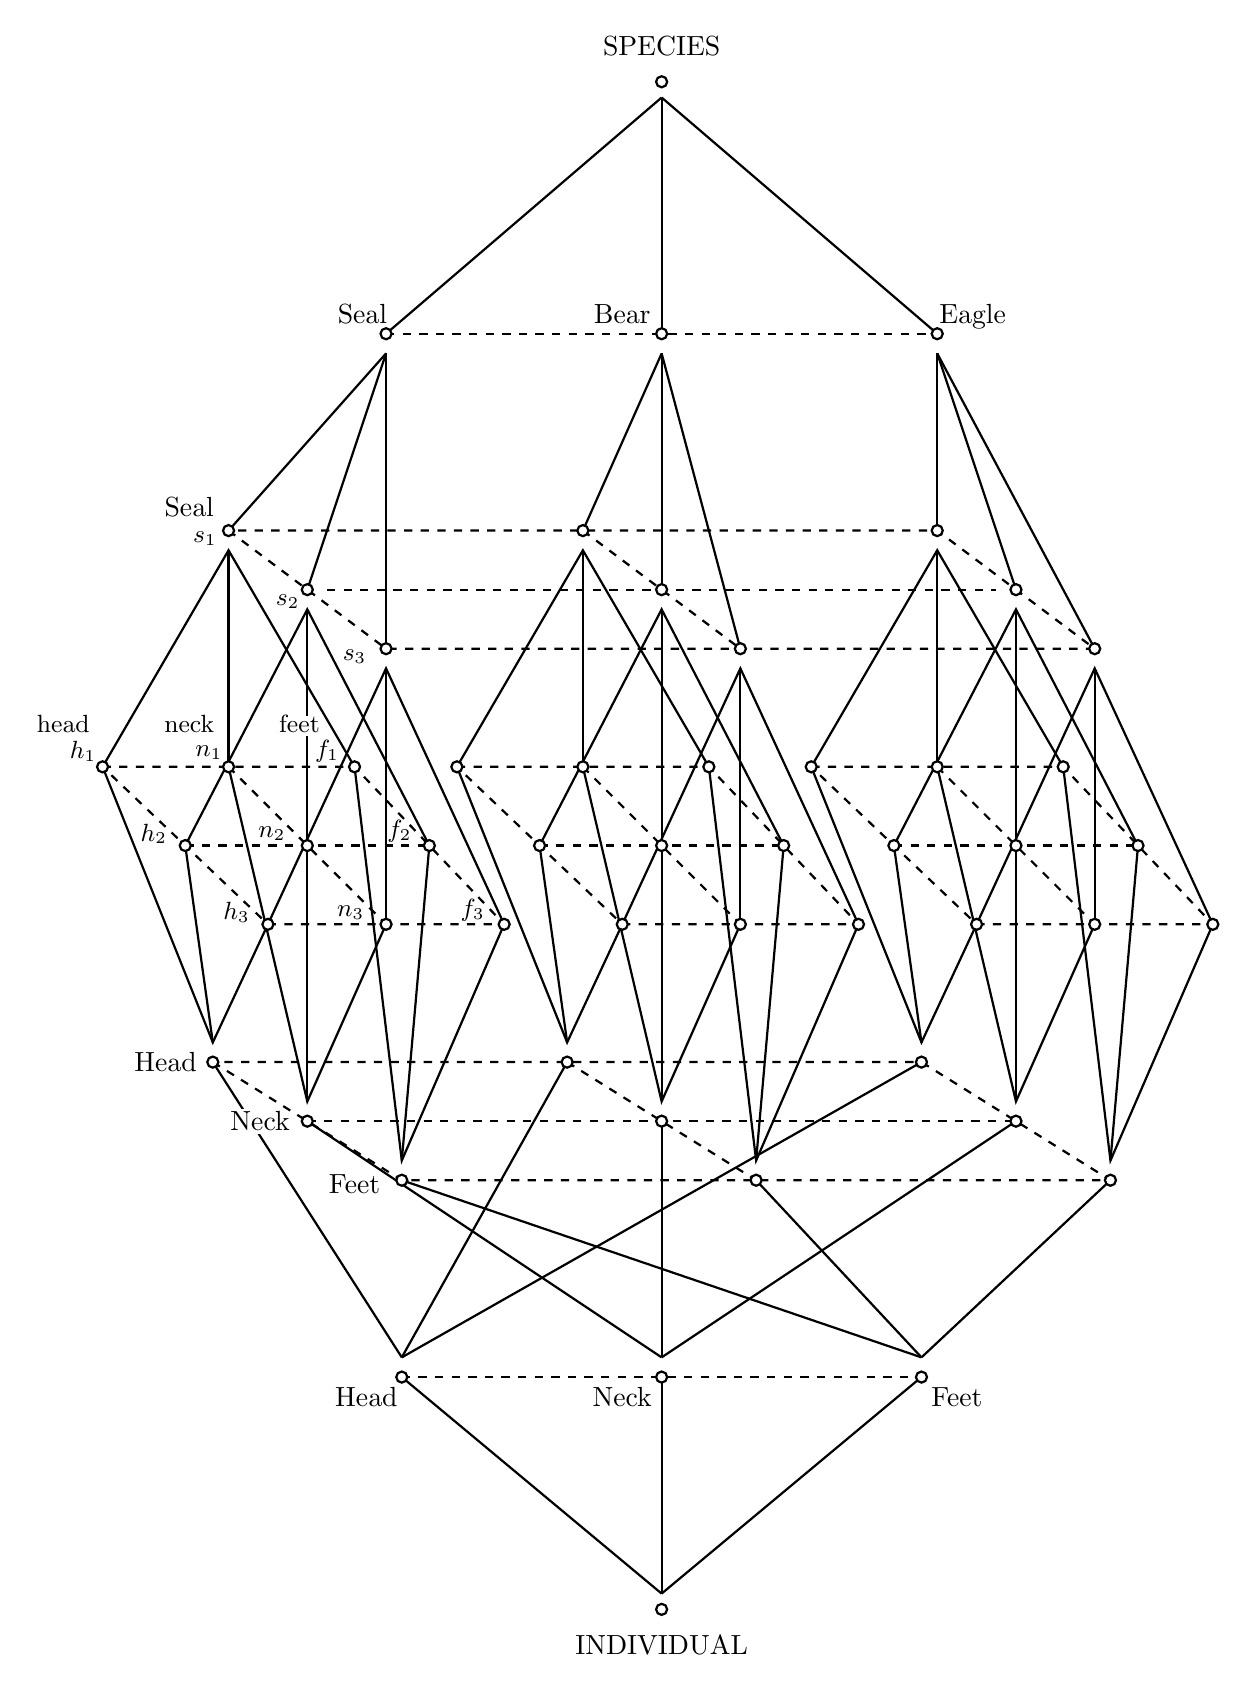
\begin{tikzpicture}
	%top labels
	\node at (0,10.15) 	  {SPECIES};
	\node at (-3.8,6.75)  {Seal};
	\node at (-0.5,6.75)  {Bear};
	\node at (3.95,6.72)  {Eagle};
	%
	\node at (-6,4.3)	 {Seal};
	\node at (-5.8,3.9)  {\small $s_1$};
	\node at (-4.75,3.1) {\small $s_2$};
	\node at (-3.9,2.4)  {\small $s_3$};
	
	%topmost triangle
	\draw[thick] (0,9.5)--(-3.5,6.5);
	\draw[thick] (0,9.5)--(0,6.5);
	\draw[thick] (0,9.5)--(3.5,6.5);
	\draw[thick,dashed] (-3.5,6.5)--(3.5,6.5);
	\filldraw[fill=white,thick] (0,9.7) circle (2pt);		%top vertex
	\filldraw[fill=white,thick] (-3.5,6.5) circle (2pt);
	\filldraw[fill=white,thick] (0,6.5) circle (2pt);
	\filldraw[fill=white,thick] (3.5,6.5) circle (2pt);
	
	%top 3 triangles
	\draw[thick] (-5.5,4)--(-3.5,6.25);		%left triangle
	\draw[thick] (-4.5,3.25)--(-3.5,6.25);
	\draw[thick] (-3.5,2.5)--(-3.5,6.25);
	\draw[thick] (-1,4)--(0,6.25);			%mid triangle
	\draw[thick] (0,3.25)--(0,6.25);
	\draw[thick] (1,2.5)--(0,6.25);
	\draw[thick] (3.5,4)--(3.5,6.25);		%right triangle
	\draw[thick] (4.5,3.25)--(3.5,6.25);
	\draw[thick] (5.5,2.5)--(3.5,6.25);
	
	%top big parallelogram
	\draw[thick,dashed] (-5.5,4)--(-3.5,2.5)--(5.5,2.5)--(3.5,4)--cycle;
	\draw[thick,dashed] (-1,4)--(1,2.5);			%horizontal dash
	\draw[thick,dashed] (-4.25,3.25)--(4.25,3.25);	%diagonal dash
	\filldraw[fill=white,thick] (-5.5,4) circle (2pt);		%left side
	\filldraw[fill=white,thick] (-4.5,3.25) circle (2pt);
	\filldraw[fill=white,thick] (-3.5,2.5) circle (2pt);
	\filldraw[fill=white,thick] (-1,4) circle (2pt);		%middle
	\filldraw[fill=white,thick] (0,3.25) circle (2pt);
	\filldraw[fill=white,thick] (1,2.5) circle (2pt);
	\filldraw[fill=white,thick] (3.5,4) circle (2pt);		%right side
	\filldraw[fill=white,thick] (4.5,3.25) circle (2pt);
	\filldraw[fill=white,thick] (5.5,2.5) circle (2pt);
	
	%left parallelogram - triangles
	\draw[thick] (-7.1,1)--(-5.5,3.75)--(-3.9,1);		%top-back
		\draw[thick] (-5.5,3.75)--(-5.5,1);
	\draw[thick] (-6.05,0)--(-4.5,3)--(-2.95,0);
		\draw[thick] (-4.5,3)--(-4.5,0);
	\draw[thick] (-5,-1)--(-3.5,2.25)--(-2,-1);
		\draw[thick] (-3.5,2.25)--(-3.5,-1);
	%
	\draw[thick] (-7.1,1)--(-5.7,-2.5)--(-5,-1);		%bot-left
		\draw[thick] (-6.05,0)--(-5.7,-2.5);
	\draw[thick] (-5.5,1)--(-4.5,-3.25)--(-3.5,-1);		%bot-mid
		\draw[thick] (-4.5,0)--(-4.5,-3.25);
	\draw[thick] (-3.9,1)--(-3.3,-4)--(-2,-1);			%bot-right
		\draw[thick] (-2.95,0)--(-3.3,-4);
		
	%left parallelogram
	\draw[thick,dashed] (-7.1,1)--(-3.9,1)--(-2,-1)--(-5,-1)--cycle;
	\draw[thick,dashed] (-6.05,0)--(-2.95,0);		%horizontal dash
	\draw[thick,dashed] (-5.5,1)--(-3.5,-1);		%diagonal dash
	\filldraw[fill=white,thick] (-7.1,1) circle (2pt);		%top row
	\filldraw[fill=white,thick] (-5.5,1) circle (2pt);
	\filldraw[fill=white,thick] (-3.9,1) circle (2pt);
	\filldraw[fill=white,thick] (-6.05,0) circle (2pt);		%mid row
	\filldraw[fill=white,thick] (-4.5,0) circle (2pt);
	\filldraw[fill=white,thick] (-2.95,0) circle (2pt);
	\filldraw[fill=white,thick] (-5,-1) circle (2pt);		%bot row
	\filldraw[fill=white,thick] (-3.5,-1) circle (2pt);
	\filldraw[fill=white,thick] (-2,-1) circle (2pt);
	
	%middle parallelogram - triangles
	\draw[thick] (-2.6,1)--(-1.0,3.75)--(0.6,1);	%top-back
		\draw[thick] (-1.0,1)--(-1.0,3.75);		%vertical line
	\draw[thick] (-1.55,0)--(0,3)--(1.55,0);		%top-mid
		\draw[thick] (0,0)--(0,3);
	\draw[thick] (-0.5,-1)--(1.0,2.25)--(2.5,-1);	%top-front
		\draw[thick] (1.0,-1)--(1.0,2.25);
	%
	\draw[thick] (-2.6,1)--(-1.2,-2.5)--(-0.5,-1);		%bot-left
		\draw[thick] (-1.55,0)--(-1.2,-2.5);
	\draw[thick] (-1.0,1)--(0,-3.25)--(1.0,-1);			%bot-mid
		\draw[thick] (0,0)--(0,-3.25);
	\draw[thick] (0.6,1)--(1.2,-4)--(2.5,-1);			%bot-right
		\draw[thick] (1.55,0)--(1.2,-4);
	
	%middle parallelogram
	\draw[thick,dashed] (-2.6,1)--(0.6,1)--(2.5,-1)--(-0.5,-1)--cycle;
	\draw[thick,dashed] (-1.55,0)--(1.55,0);	%horizontal dash
	\draw[thick,dashed] (-1,1)--(1,-1);			%diagonal dash
	\filldraw[fill=white,thick] (-2.6,1) circle (2pt);		%top row
	\filldraw[fill=white,thick] (-1,1) circle (2pt);
	\filldraw[fill=white,thick] (0.6,1) circle (2pt);
	\filldraw[fill=white,thick] (-1.55,0) circle (2pt);		%mid row
	\filldraw[fill=white,thick] (0,0) circle (2pt);
	\filldraw[fill=white,thick] (1.55,0) circle (2pt);
	\filldraw[fill=white,thick] (-0.5,-1) circle (2pt);		%bot row
	\filldraw[fill=white,thick] (1.0,-1) circle (2pt);
	\filldraw[fill=white,thick] (2.5,-1) circle (2pt);
	
	%right parallelogram - triangles
	\draw[thick] (1.9,1)--(3.5,3.75)--(5.1,1);		%top-back
		\draw[thick] (3.5,1)--(3.5,3.75);		%vertical line
	\draw[thick] (2.95,0)--(4.5,3)--(6.05,0);		%top-mid
		\draw[thick] (4.5,0)--(4.5,3);
	\draw[thick] (4,-1)--(5.5,2.25)--(7,-1);		%top-front
		\draw[thick] (5.5,-1)--(5.5,2.25);
	%
	\draw[thick] (1.9,1)--(3.3,-2.5)--(4,-1);		%bot-left
		\draw[thick] (2.95,0)--(3.3,-2.5);
	\draw[thick] (3.5,1)--(4.5,-3.25)--(5.5,-1);	%bot-mid
		\draw[thick] (4.5,0)--(4.5,-3.25);
	\draw[thick] (5.1,1)--(5.7,-4)--(7,-1);			%bot-right
		\draw[thick] (6.05,0)--(5.7,-4);
	
	%right parallelogram
	\draw[thick,dashed] (1.9,1)--(5.1,1)--(7,-1)--(4,-1)--cycle;
	\draw[thick,dashed] (2.95,0)--(6.05,0);		%horizontal dash
	\draw[thick,dashed] (3.5,1)--(5.5,-1);		%diagonal dash
	\filldraw[fill=white,thick] (1.9,1) circle (2pt);		%top row
	\filldraw[fill=white,thick] (3.5,1) circle (2pt);
	\filldraw[fill=white,thick] (5.1,1) circle (2pt);
	\filldraw[fill=white,thick] (2.95,0) circle (2pt);		%mid row
	\filldraw[fill=white,thick] (4.5,0) circle (2pt);
	\filldraw[fill=white,thick] (6.05,0) circle (2pt);
	\filldraw[fill=white,thick] (4,-1) circle (2pt);		%bot row
	\filldraw[fill=white,thick] (5.5,-1) circle (2pt);
	\filldraw[fill=white,thick] (7,-1) circle (2pt);
	
	%center labels
	\node at (-7.35,1.2)   {\small $h_1$};
	\node at (-6.45,0.15)  {\small $h_2$};
	\node at (-5.40,-0.85) {\small $h_3$};
	%
	\node at (-5.75,1.18)  {\small $n_1$};
	\node at (-4.95,0.15)  {\small $n_2$};
	\node at (-3.95,-0.85) {\small $n_3$};
	%
	\node at (-4.25,1.2)  {\small $f_1$};
	\node at (-3.33,0.18) {\small $f_2$};
	\node at (-2.4,-0.82) {\small $f_3$};
	%
	\node at (-7.6,1.55) {\small head};
	\node at (-6.0,1.55) {\small neck};
	\draw[line width=7pt,color=white] (-4.8,1.52)--(-4.4,1.52);	%manual fill for `feet'
	\node at (-4.6,1.55) {\small feet};
	
	%bottom interscrossings
	\draw[thick] (-3.3,-6.5)--(-5.7,-2.75);		%from left vertex
	\draw[thick] (-3.3,-6.5)--(-1.2,-2.75);
	\draw[thick] (-3.3,-6.5)--(3.3,-2.75);
	\draw[thick] (0,-6.5)--(-4.5,-3.5);			%from middle vertex
	\draw[thick] (0,-6.5)--(0,-3.5);
	\draw[thick] (0,-6.5)--(4.5,-3.5);
	\draw[thick] (3.3,-6.5)--(-3.3,-4.25);		%from right vertex
	\draw[thick] (3.3,-6.5)--(1.2,-4.25);
	\draw[thick] (3.3,-6.5)--(5.7,-4.25);
	
	%bottom big parallelogram
	\draw[thick,dashed] (-5.7,-2.75)--(-3.3,-4.25)--(5.7,-4.25)--(3.3,-2.75)--cycle;
	\draw[thick,dashed] (-1.2,-2.75)--(1.2,-4.25);		%horizontal dash
	\draw[thick,dashed] (-4.5,-3.5)--(4.5,-3.5);		%diagonal dash
	\filldraw[fill=white,thick] (-5.7,-2.75) circle (2pt);		%left side
	\filldraw[fill=white,thick] (-4.5,-3.5) circle (2pt);
	\filldraw[fill=white,thick] (-3.3,-4.25) circle (2pt);
	\filldraw[fill=white,thick] (-1.2,-2.75) circle (2pt);		%middle
	\filldraw[fill=white,thick] (0,-3.5) circle (2pt);
	\filldraw[fill=white,thick] (1.2,-4.25) circle (2pt);
	\filldraw[fill=white,thick] (3.3,-2.75) circle (2pt);		%right side
	\filldraw[fill=white,thick] (4.5,-3.5) circle (2pt);
	\filldraw[fill=white,thick] (5.7,-4.25) circle (2pt);
	
	%bottommost triangle
	\draw[thick,dashed] (-3.3,-6.75)--(3.3,-6.75);
	\draw[thick] (0,-9.5)--(-3.3,-6.75);
	\draw[thick] (0,-9.5)--(0,-6.75);
	\draw[thick] (0,-9.5)--(3.3,-6.75);
	\filldraw[fill=white,thick] (-3.3,-6.75) circle (2pt);
	\filldraw[fill=white,thick] (0,-6.75) circle (2pt);
	\filldraw[fill=white,thick] (3.3,-6.75) circle (2pt);
	\filldraw[fill=white,thick] (0,-9.7) circle (2pt);		%bottom vertex
	
	%bottom labels
	\node at (-6.3,-2.75) {Head};
	\draw[line width=9pt,color=white] (-5.5,-3.5)--(-5,-3.5);	%manual fill for `neck'
	\node at (-5.1,-3.5)  {Neck};
	\node at (-3.9,-4.3)  {Feet};
	%
	\node at (-3.75,-7) {Head};
	\node at (-0.5,-7)  {Neck};
	\node at (3.75,-7)  {Feet};
	\node at (0,-10.15) {INDIVIDUAL};
	%\draw[help lines] (-8,10) grid (8,-10);
	\end{tikzpicture}
	%	\caption{The totemic operator}
	%\end{figure}
	
	
	\vspace{2cm}
	
	
	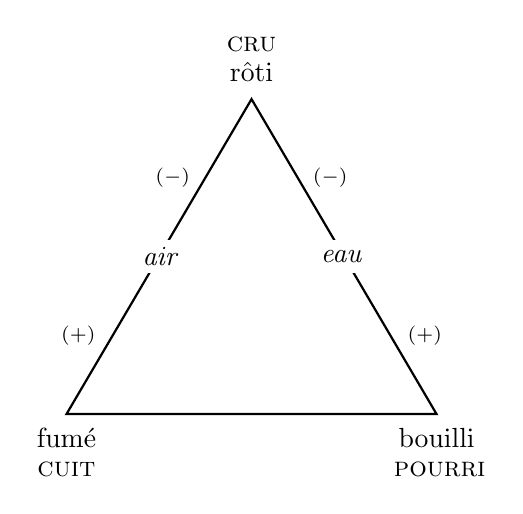
\begin{tikzpicture}
	%lines
	\draw[thick] (0,0)--(-2.35,-4)--(2.35,-4)--cycle;
	
	%labels
	\node at (0,0.35) 	  {r\^{o}ti};
	\node at (0,0.7) 	  {\textsc{cru}};
	\node at (-2.35,-4.3) {fum\'{e}};
	\node at (-2.35,-4.7) {\textsc{cuit}};
	\node at (2.35,-4.3)  {bouilli};
	\node at (2.39,-4.7)  {\textsc{pourri}};
	%
	\draw[line width=12pt, color=white] (-1.5,-2)--(-0.5,-2);	%manual fill
	\draw[line width=12pt, color=white] (1.5,-2)--(0.5,-2);
	\node at (-1.15,-2) {\textit{air}};
	\node at (1.15,-2)  {\textit{eau}};
	%
	\node at (-1,-1)   {\scriptsize $(-)$};
	\node at (1,-1)    {\scriptsize $(-)$};
	\node at (-2.2,-3) {\scriptsize $(+)$};
	\node at (2.2,-3)  {\scriptsize $(+)$};
	%\draw[help lines] (-3,-5) grid (3,1);
	\end{tikzpicture}
	%
	%
	\hspace{1.5cm}%
	%
	%
	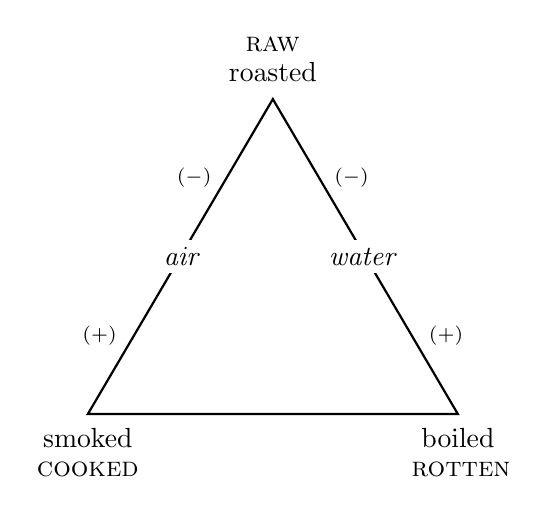
\begin{tikzpicture}
	%lines
	\draw[thick] (0,0)--(-2.35,-4)--(2.35,-4)--cycle;
	
	%labels
	\node at (0,0.35) 	  {roasted};
	\node at (0,0.7) 	  {\textsc{raw}};
	\node at (-2.35,-4.3) {smoked};
	\node at (-2.35,-4.7) {\textsc{cooked}};
	\node at (2.35,-4.3)  {boiled};
	\node at (2.39,-4.7)  {\textsc{rotten}};
	%
	\draw[line width=12pt, color=white] (-1.5,-2)--(-0.5,-2);	%manual fill
	\draw[line width=12pt, color=white] (1.5,-2)--(0.5,-2);
	\node at (-1.15,-2) {\textit{air}};
	\node at (1.15,-2)  {\textit{water}};
	%
	\node at (-1,-1)   {\scriptsize $(-)$};
	\node at (1,-1)    {\scriptsize $(-)$};
	\node at (-2.2,-3) {\scriptsize $(+)$};
	\node at (2.2,-3)  {\scriptsize $(+)$};
	%\draw[help lines] (-3,-5) grid (3,1);
	\end{tikzpicture}
	
\end{document}